\documentclass[sigconf]{acmart}

\sloppy
\settopmatter{printacmref=false} % Removes citation information below abstract
\renewcommand\footnotetextcopyrightpermission[1]{} % removes footnote with conference information in first column
\pagestyle{plain} % removes running headers
\usepackage{booktabs} % For formal tables
\usepackage{caption}
\usepackage{subcaption}
% Rights management information. 
% This information is sent to you when you complete the rights form.
% These commands have SAMPLE values in them; it is your responsibility as an author to replace
% the commands and values with those provided to you when you complete the rights form.
%
% These commands are for a PROCEEDINGS abstract or paper.
% \copyrightyear{2018}
% \acmYear{2018}
% \setcopyright{acmlicensed}
% \acmConference[Woodstock '18]{Woodstock '18: ACM Symposium on Neural Gaze Detection}{June 03--05, 2018}{Woodstock, NY}
% \acmBooktitle{Woodstock '18: ACM Symposium on Neural Gaze Detection, June 03--05, 2018, Woodstock, NY}
% \acmPrice{15.00}
% \acmDOI{10.1145/1122445.1122456}
% \acmISBN{978-1-4503-9999-9/18/06}

%
% These commands are for a JOURNAL article.
%\setcopyright{acmcopyright}
%\acmJournal{TOG}
%\acmYear{2018}\acmVolume{37}\acmNumber{4}\acmArticle{111}\acmMonth{8}
%\acmDOI{10.1145/1122445.1122456}

%
% Submission ID. 
% Use this when submitting an article to a sponsored event. You'll receive a unique submission ID from the organizers
% of the event, and this ID should be used as the parameter to this command.
%\acmSubmissionID{123-A56-BU3}

%
% The majority of ACM publications use numbered citations and references. If you are preparing content for an event
% sponsored by ACM SIGGRAPH, you must use the "author year" style of citations and references. Uncommenting
% the next command will enable that style.
%\citestyle{acmauthoryear}

%
% end of the preamble, start of the body of the document source.
\begin{document}\Large
%

\title{Automatic Generate Title Of Articles From Newspaper}

%
% The "author" command and its associated commands are used to define the authors and their affiliations.
% Of note is the shared affiliation of the first two authors, and the "authornote" and "authornotemark" commands
% used to denote shared contribution to the research.
\author{Your Name}

\email{email@stevens.edu}
\orcid{1234-5678-9012}
\affiliation{%
  \institution{Stevens Institution of Technology}
  \streetaddress{1 Castle Point Terrace}
  \city{Hoboken}
  \state{NJ}
  \postcode{07030}
}



% By default, the full list of authors will be used in the page headers. Often, this list is too long, and will overlap
% other information printed in the page headers. This command allows the author to define a more concise list
% of authors' names for this purpose.
% \renewcommand{\shortauthors}{Trovato and Tobin, et al.}


%
% This command processes the author and affiliation and title information and builds
% the first part of the formatted document.
\begin{abstract}
Text summarization refers to the technique of shortening long pieces of text. The intention is to create a coherent and fluent summary having only the main points outlined in the document. Automatic text summarization is a common problem in machine learning and natural language processing (NLP). In our project, we optimize four different parts on the traditional seq2seq model. First, the length of input text. Second, the ratio of teacher forcing during training process. Third, find a better attention method which is more useful to our model. Forth, find a better K when we use beam search to generate outputs. 
\end{abstract}
\maketitle


\section{Introduction}
In recent decades, text summarization has become a popular topic in natural language processing field. The reason is redundancy in large text collections will cause difficulties for the users of search engines if there are too many similar information on the website. So that these people need to read and search time and time again. However, this problem can also be a good thing which can be used to identify important information, such as summarization and question answering.

There are two main approaches to automatic summarization: extraction and abstraction. Extraction method is find some words, phrases or some sentences which are existing in the paragraph. Extraction method is build an internal semantic representation, then the model will generate a summary by natural language generation techniques which is more closer to what human might express.

In our project, we build a Deep Neural Networks which base on the sequence to sequence model which has two RNN parts in it, encoder model and decode model. The goal of encoder model is learn the input text and transfer them into different vectors which can represent the input and can be calculated by computer. Similarly, decoder model's task is translate these vectors into sentences which can be read by human.

\section{Related Work}
\subsection{Encoder and Decoder}
We have talked about the main task of encoder and decoder model in previous section. And in this section, we will show how we optimize these two models. Firstly, in the original encoder model, all the input text have the same length, no matter use the mean length of all data or just use the maximum length. 

It means if the length of a paragraph larger than the standard length, extra part of this paragraph will be ignore. It would cause a problem that encoder model lose some information, as a result, the output vector couldn't represent the data perfectly. On the other hand, if the length of a paragraph less than the standard length, the model will add 0 until the length of input is equal to standard length. Similarly, the problem is the model will receive many useless information which may waste time. So, what we want to do is skip these useless time step during training process.

\subsection{Teacher Forcing}
Teacher forcing is a method for quickly and efficiently training recurrent neural network models that use the ground truth from a prior time step as input. It is a network training method critical to the development of deep learning language models used in machine translation, text summarization, and image captioning, among many other applications. In our project, we want to find a ratio of teacher forcing which means, some time steps use this technology, other time steps don't use it.

\subsection{Attention}
Attention is a mechanism that was developed to improve the performance of the Encoder-Decoder RNN on machine translation. And it is proposed as a solution to the limitation of the Encoder-Decoder model encoding the input sequence to one fixed length vector from which to decode each output time step. This issue is believed to be more of a problem when decoding long sequences. In out project, we will implement two different attention model, Bahdanaua and Luong. The previous structure is using last hidden state compute the weight of attention section and the latter one is using current hidden state to compute the weight of attention section. We will find a better method to get a higher performance. 

\subsection{Beam Search}
In computer science, beam search is a heuristic search algorithm that explores a graph by expanding the most promising node in a limited set. Beam search is an optimization of best-first search that reduces its memory requirements. Best-first search is a graph search which orders all partial solutions (states) according to some heuristic. But in beam search, only a predetermined number of best partial solutions are kept as candidates. It is thus a greedy algorithm. In our project, we will implement this technology and find a best k which has the best performance.

\begin{figure}
    \centering
    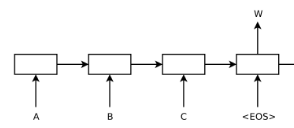
\includegraphics[width = 2.8in, height = 1.3in]{encoder.png}
    \caption{structure of encoder and decoder}
    \label{fig:1}
\end{figure}
\begin{figure}
    \centering
    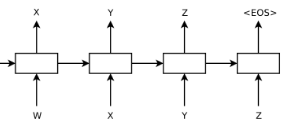
\includegraphics[width = 2.8in, height = 1.3in]{decoder.png}
    \caption{structure of encoder and decoder}
    \label{fig:2}
\end{figure}
\begin{figure}
    \centering
    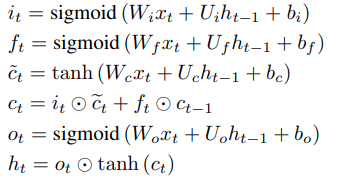
\includegraphics[width = 2.7in, height = 1.3in]{LSTM.png}
    \caption{functions of LSTM}
    \label{fig:3}
\end{figure}
\section{Methods}
\subsection{Structure of Encoder and Decoder}
In our project, we implement this model by tensorflow, and the base structure of encoder and decoder are shown as figure 1 and figure 2. The first four time steps are encoder part and the other time steps are decoder part. No matter encoder or decoder, all of them are LSTM model. Long short-term memory (LSTM) is an artificial recurrent neural network (RNN) architecture used in the field of deep learning. Unlike standard feed forward neural networks, LSTM has feedback connections. It can not only process single data points, but also entire sequences of data. a memory state c, an output gate o, as well as an input gate i and a forget gate f. The updates are parameterised by eight weight matrices associated with these (four W, and four U) as well as biases.The main functions of LSTM are shown in figure 3.

\begin{figure}
    \centering
    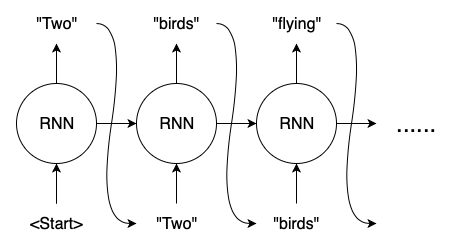
\includegraphics[width = 2.7in, height = 1.3in]{with_teacher_forcing.png}
    \caption{without teacher forcing}
    \label{fig:4}
\end{figure}

\begin{figure}
    \centering
    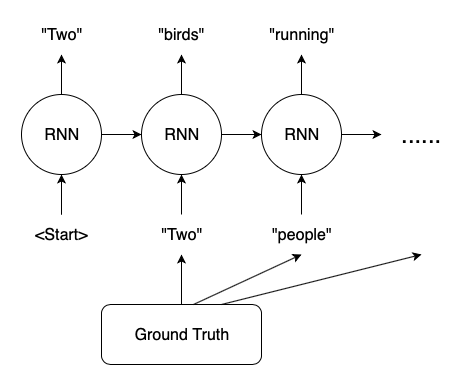
\includegraphics[width = 2.7in, height = 1.8in]{without_teacher_forcing.png}
    \caption{with teacher forcing}
    \label{fig:5}
\end{figure}
\subsection{Teacher Forcing}
Teacher forcing is the technique where the target word is passed as the next input to the decoder. Figure 4 and figure 5 shows the model with teacher forcing and without teacher forcing. Training with Teacher Forcing converges faster. At the early stages of training, the predictions of the model are very bad. If we do not use Teacher Forcing, the hidden states of the model will be updated by a sequence of wrong predictions, errors will accumulate, and it is difficult for the model to learn from that.

\subsection{Attention}
Attention was presented by Dzmitry Bahdanau, et al. in their paper “Neural Machine Translation by Jointly Learning to Align and Translate” that reads as a natural extension of their previous work on the Encoder-Decoder model. Instead of encoding the input sequence into a single fixed context vector, the attention model develops a context vector that is filtered specifically for each output time step. There are many main attention mechanism, and we will implement two of them. One is Bahdanau, another one is Luong.
\begin{figure}
    \centering
    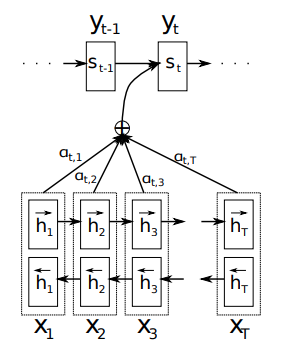
\includegraphics[width = 1.9in, height = 1.8in]{bahda.png}
    \caption{Bahdanau}
    \label{fig:6}
\end{figure}

\begin{figure}
    \centering
    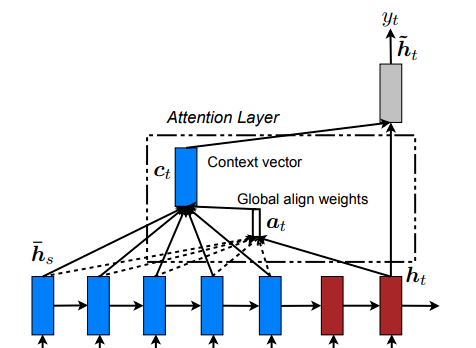
\includegraphics[width = 2.7in, height = 1.8in]{luong.png}
    \caption{Luong}
    \label{fig:7}
\end{figure}
\subsubsection{Bahdanaua}

The structure of Bahdanaua is shown in figure 6. The ith Target word context vector c-i will be based on the hidden vector of each source word h-j weighted summation yields: $$C_i=\sum_{j=1}^{Tx}\alpha_{ij}h_{j}$$
For each h-j of a-ij calculated as follows:
$$\alpha_{ij} = \frac{exp(e_{ij})}{\sum_{k=1}^{Tx}(exp(e_{ik}))}$$
among them:
$$e_{ij} = a(s_{i-1},h_j)$$
$e_{ij}$ is the alignment model, representing the position j input and location i. The output matches the score of the degree based on the implied state of the i-1 position of the RNN $s_{i-1}$ dnd j position $h_{j}$ calculated.
\subsubsection{Luong}
Luong attention is described in the thesis “Effective Approaches to Attention-based Neural Machine Translation”. Its structure is shown in figure 7. Similar to the overall structure of Bahdanau Attention, Luong attention makes some adjustments to the original structure, and the attention vector is calculated as follows:
$$a_t(s) = \frac{exp(score(h_t,\bar{h_s}))}{\sum_{s'}^{}exp(score(h_t,\bar{h_s_'}))}$$
The calculation flow of Bahdanaua attention is:
$$h_{t-1} \rightarrow a_t\rightarrow c_t\rightarrow h_t$$
The Luong attention calculation process is:
$$h_t \rightarrow a_t\rightarrow c_t\rightarrow \widetilde{h_t}$$

\subsection{Beam Search}
There is a better way of performing decoding, called Beam Search. Instead of only predicting the token with the best score, we keep track of k hypotheses (for example k = 3, we refer to k as the beam size). At each new time step, for these k hypotheses we have V new possible tokens. It makes a total of kV new hypotheses. Then, only keep the 5 best ones, and so on.... 
$H_t$ is the set of hypotheses decoded at time step t:
$$H_t := \left \{ (w_1^1,...,w_t^1),...,(w_1^k,...,w_t^k) \right \}$$
For example, if k = 2, one possible H is:
$$H_t := \left \{ (a,b),(a,c) \right \}$$
So, all the possible candidates:
$$A_{t+1} := \bigcup_{i=1}^{k} = \left \{(w_1^i,...w_t^i,1),...(w_1^i,...,w_t^i,V) \right \}$$
Than, if t = 2:
$$A_3 = \left \{  (a,b,a),(a,b,b),(a,b,c)\right \}\cup \left \{ (a,c,a),(a,c,b),(a,c,c)) \right \}$$
Once every hypothesis reached the <eos> token, we return the hypothesis with the highest score.
\section{Experimental Evaluation}


\bibliographystyle{ACM-Reference-Format}
\bibliography{sample-base}

\end{document}
